\documentclass[10pt,a4paper]{article}
\usepackage[utf8]{inputenc}
\usepackage{amsmath}
\usepackage{amsfonts}
\usepackage{amssymb}
\usepackage{geometry}
\geometry{margin=1in}
\usepackage{hyperref}
\hypersetup{
     colorlinks = true,
     linkcolor = blue,
     }
\usepackage{graphicx}
\usepackage[bottom]{footmisc} 
\usepackage{floatrow}
\usepackage[utf8]{inputenc}
\usepackage[round]{natbib}
\usepackage{booktabs}
\usepackage{array}
\hypersetup{citecolor=black}

\begin{document}

\begin{center}
\textbf{{\LARGE Macroeconomic Model Data Base 3.1.0 User Guide}}
\end{center}
\bigskip
This manual guides users through the Macroeconomic Model Data Base (MMB hereafter) 3.1.0 version, which includes 151 models. Chapter 1 explains the required software and basic setting to run the MMB; chapter 2 introduces the MMB interface, chapter 3 the key folder and files that govern simulation in the MMB. Two new features are illustrated in chapter 4 and 5: add new models and new policy rules. All the instructions in the user guide apply to Windows, macOS and Linux.
\medskip

\begin{flushleft}
\section{Environment Setting}
\end{flushleft}
\medskip

\subsection{Required Software}
\medskip

\begin{itemize}
\item Please install either \textbf{MATLAB} or \textbf{Octave} to simulate models on the MMB. For MATLAB, the \textit{Optimization Toolbox} package, the \textit{Statistics Toolbox} package and the R2019a or newer versions are required. For Octave, the \textit{statistics} package, the \textit{io} package and the 4.4.1 or the 5.1 version are required.

\item Please install \textbf{Dynare} to solve models on the MMB, which supports the 4.5.6 and the 4.5.7 versions.\footnote{Please note that earlier versions of Dynare were not tested on the MMB 3.1.0 but may work as well.}

\item Please go to \url{https://www.dynare.org/resources/quick_start/} for instructions to set up your Dynare in MATLAB or Octave.
\end{itemize}

\subsection{Settings}
\medskip

\begin{itemize}
\item Please specify that either MATLAB or Octave is used on the MMB. At the upper-right corner of the MMB interface, click ‘Menu’ $>$ ‘Setting’ and then a window will pop out for users to either click ‘Scan’ to let the MMB automatically search for MATLAB/Octave, or click ‘Find manually’ . If MATLAB/Octave cannot be found through scan, users then need to find the software manually.

\item If users clicked ‘Scan’, MMB may find more than one version of MATLAB/Octave — click the white bar to choose which version to use.\footnote{Please note that the MMB only scans common directories for time saving.}

\item If users clicked ‘Find manually’, a window will pop out for users to add either MATLAB or Octave. For MATLAB, please browse your directory all the way to ‘.../matlab/version/bin/matlab.exe’. For Octave, please browse your directory all the way to ‘.../octav/version/bin/octave-cli.exe’.

\item Click ‘Remove selected’ to remove MATLAB/Octave version selected.

\item Please follow the same instructions above to set up Dynare.

\item To set your path in the MMB, click ‘Use builtin’ and the directory to where the MMB package is downloaded will be located automatically. Users can also click ‘Select folder’ to locate the directory manually, or click ‘Extra file’ to load the MMB package to an empty folder.

\item Click ‘Check compatibility’ at the lower-left corner of the window to confirm whether or not the installed MATLAB/Octave is compatible with the MMB.
\end{itemize}
\pagebreak








\begin{flushleft}
\section{The Interface}
\end{flushleft}
\medskip

The MMB interface is divided into five menus: ‘Models’, ‘Policy Rules’, ‘Shocks’, ‘Variables’ and ‘Options’. Users can hover cursor over the models or the policy rules for basic academic references. For assistance, please click ‘Menu’ $ > $ ‘Help’.
\medskip

The MMB 3.1.0 features comparison of multiple models with multiple policy rules — in the previous versions, the MMB allowed only one model with multiple rules or multiple models with only one rule. More common variables and common shocks are also added to enhance the comparison exercises and users can edit the models and policy rules.
\bigskip
\bigskip

\subsection{Models}
\label{sec:Models}
\medskip

\begin{itemize}
\item The MMB categorizes the models into five groups. \textbf{‘Calibrated’} includes models calibrated to match a closed economy. \textbf{‘Estimated US’} and \textbf{‘Estimated Euro Area’} include models estimated on the US and the Euro area data. \textbf{‘Other’} includes models calibrated or estimated on data of multiple countries or countries outside the US or the Euro area, i.e., CA\_BMZ12 is a model estimated on Canadian data; EAUS\_NAWM08 is a two-economy model estimated on data of the Euro area and the US. \textbf{‘Adaptive Learning’} includes models in which agents form expectations through adaptive learning.

\item The name of a model starts with the group to which the model belongs, followed by the first letter of the model developers’ last name, and ends with the publication year, e.g., US\_SW07 stands for the model estimated on the US data and developed by \cite{SmetsWouters2007}. For adaptive learning models, “AL” is added at the end of the name, e.g., US\_SW07AL.

\item To look for a model, type keywords, e.g., author, paper title, journal name or year, in the search bar at the upper-right corner of the interface.

\item To look into details of the models, click ‘Documentation of Models’ at the bottom of the ‘Models’ menu.
\end{itemize}

\subsection{Policy Rules}
\label{sec:Rules}
\medskip

\begin{itemize}
\item The MMB offers \textbf{nine common monetary policy rules} written in a standardized equation\footnote{To see the equation, go to the section of Policy Rules in \hyperref[sec:Model]{3.2.2 The Model}.} that is consisted of the four common variables in the MMB.\footnote{See \hyperref[sec:Var]{2.4 Variables}.}

\item ‘Model specific rule’ is available if a model has a specific policy rule that can be transformed into the standardized equation used in the common monetary policy rules. For specific policy rules that cannot be transformed due to inclusion of variables other than the four common variables, e.g., exchange rate, the model has to be simulated by the common monetary policy rules. A total of 112 models can be simulated with their specific policy rules.

\item ‘User specified rule’ allows users to tailor a desired monetary policy rule. Click ‘(edit)’ and then a window will pop out for users to set the coefficients — please note that the Blanchard and Kahn condition may not be satisfied, and a determined equilibrium may not be obtained in the solution. 

\item Please note that some policy rules may fade out on the menu and cannot be selected for comparison exercises if they are not compatible with one of the selected models.
\end{itemize}

\subsection{Shocks}
\label{sec:Shocks}
\medskip

\begin{itemize}
\item The MMB offers \textbf{two common shocks}: the monetary policy shock (one percentage point increase in the interest rate) can be simulated for all the models while the fiscal policy shock (one percentage increase in the share of government expenditures in GDP) is limited to some specific models. 

\item Some other common shocks, e.g., technology shock, are also available, depending on which models are selected. Overall, when a model is selected on the menu, all the shocks defined in the model’s mod-file\footnote{See \hyperref[sec:Mod]{3.2 Mod-files}.} are listed, but only common shocks appear with a label. If two or more models are selected, only those shocks shared by the selected models appear.
\end{itemize}

\subsection{Variables}
\label{sec:Var}
\medskip

\begin{itemize}
\item The MMB offers \textbf{four common variables} and they are selected by default on the interface: output (quarterly), output gap (quarterly), inflation rate (year-on-year) and interest rate (in annualized terms).\footnote{See the section of Definition of MMB Common Variables in Terms of New Model Variables in \hyperref[sec:Model]{3.2.2 The Model} for the details.}

\item Some other common variables, e.g., consumption, are also available, depending on which models are selected. Overall, when a model is selected on the menu, all the variables defined in the model’s mod-file (see \hyperref[sec:Mod]{3.2 Mod-files}) are listed, but only common variables appear with a label. If two or more models are selected, only those variables shared by the selected models appear.
\end{itemize}

\subsection{Options}
\medskip

\begin{itemize}
\item Users can choose whether or not to plot \textbf{unconditional variances} or \textbf{autocorrelation functions}\footnote{For adaptive learning models, variances and autocorrelations are calculated by 200 simulations that use random numbers. To modify simulation number, go to ....\textbackslash lib\textbackslash stoch\_simul\_MMB.m and change the number after \textit{n\_sims}. Please note the trade-off between precision and simulation time. Variances and autocorrelation may also vary on MATLAB and Octave due to different algorithms to generate random numbers; impulse response functions, nevertheless, are not affected.} of common variables and determine the \textbf{horizon} of impulse response analysis (20 periods are set by default).\footnote{For models featuring unit roots, unconditional variances are not defined, and autocorrelation functions do not exist since unit roots prevent the calculation of some or all variables’ unconditional moments. Nonetheless, impulse response functions can still be generated.} 

\item If an adaptive learning model is selected, drag the ‘Gain’ bar to set the gain parameter and click ‘Select states’ — a window will pop out for users to select states in the model.
\end{itemize}

\subsection{Run Comparison Exercise}
\medskip

\begin{itemize}
\item Click ‘Compare’ after selecting models, policy rules, shocks, variables and other options and a window will pop up, showing that MATLAB or Octave\footnote{Octave may take much longer time than MATLAB.} is simulating the model(s). Once the simulation is done, click ‘Close’ to see the results, which appear at the bottom of the MMB interface.\footnote{Users may need to scroll down the interface to see the results.}

\item The MMB displays the results by variables, but users can click ‘Group Data’ to display the results in terms of model or policy rule. Users can also click elements in the legend to choose which variables, models or policy rules to display and drag the bar of ‘Max number column per row’ for desired display of the results. See Figure 2.1.

\item To export the results, either click ‘CSV’ or ‘JSON’ to save all the results at once, or click the menu icon at the upper-right corner of each figure to save the results individually. See Figure 2.1.
\end{itemize}

\subsection{Edit Model and Policy Rules}
\medskip

\begin{itemize}
\item To edit the models and policy rules, e.g., renaming a variable or a shock, click ‘Menu’ $>$ ‘Edit Model Rules/Models’ and a window will pop out, showing a list of all the models in the MMB. Click the model to edit its mod-file or json-file — see the following chapters for details. Click ‘Save’ every time finishing your edits and before moving on to the next model. Click ‘Close’ and ‘Menu’ $>$ ‘Reload Data’ to apply the edits.
\end{itemize}
\pagebreak

\begin{center}
Figure 2.1: Run Comparison Exercises\\
\medskip
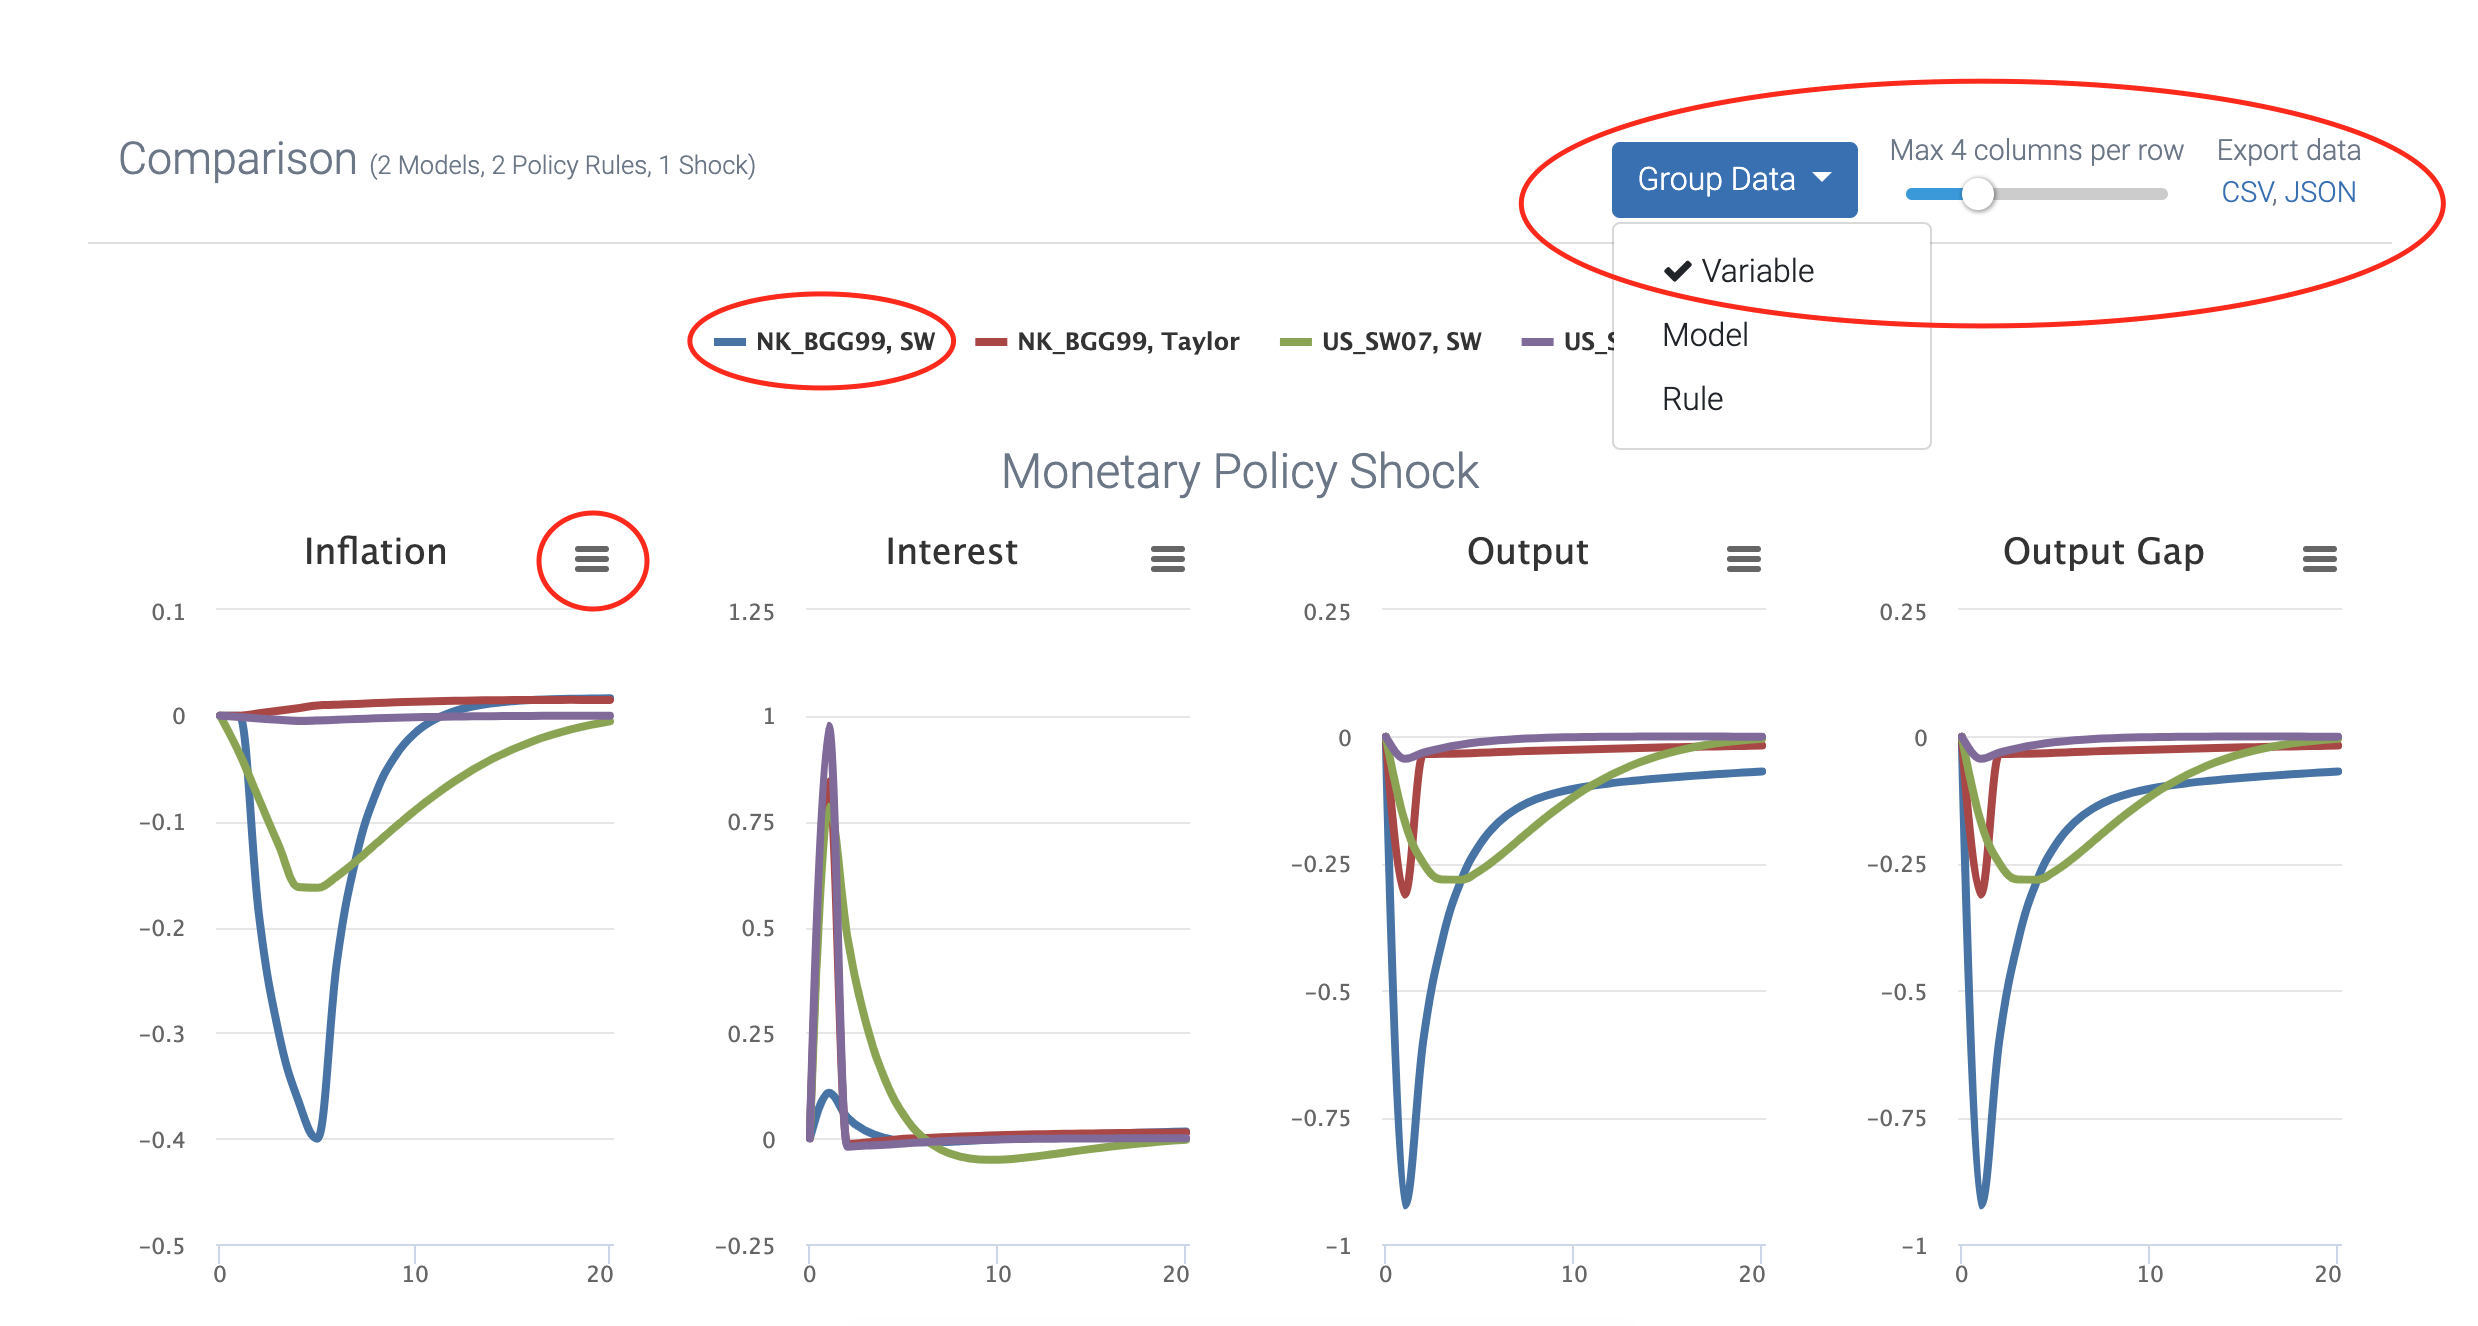
\includegraphics[scale=0.35]{group}
\end{center}
\bigskip

\pagebreak








\begin{flushleft}
\section{Folders and Files}
\end{flushleft}
\medskip


\subsection{Key Folders}
\medskip

\begin{itemize}
\item The \textbf{\textit{models}} folder\footnote{All the folders and files introduced in this chapter are here: Resources\textbackslash app\textbackslash dist\textbackslash electron\textbackslash static\textbackslash mmci-cli. For macOS users, please right click the MMB in Finder and click ‘Show Package Content’ to browse the folders and the files.} contains a list of folders for all the models in the MMB and each of these folders has one \textbf{mod-file} written in Dynare syntax, one \textbf{json-file} that links the mod-file and the interface and, for models with non-zero steady states, one or more \textbf{m-file}(s) that contains the steady-state equations or values — see \hyperref[sec:Mod]{3.2 Mod-files} and \hyperref[sec:Json]{3.3 Json-files}. 

\item The \textbf{\textit{rules}} folder contains a list of folders for the nine common monetary policy rules in the MMB and each of these folders has one json-file. 

\item The \textbf{\textit{lib\textbackslash ALTOOLS}} folder contains a list of scripts for adaptive learning models.
\end{itemize}

\subsection{Mod-files}
\label{sec:Mod}
\bigskip

A mod-file starts with some basic information about the model, followed by \textbf{two blocks}: the preamble and the model.

\subsubsection{The Preamble}
\label{sec:Preamble}
\medskip

\begin{itemize}
\item The preamble block is consisted of \textbf{seven sections}. Sections introduced below with an asterisk * indicates those written for the compatibility with the MMB and are separated by slashes and asterisks \texttt{//********}.

\item The section of \textbf{var} lists endogenous variables in the model. Please note that the notation for a model's fiscal shock is also defined as an endogenous variable here, e.g., \texttt{g\_} in NK\_RW97. This is because MMB already has a built-in fiscal policy shock,\footnote{See \hyperref[sec:Shocks]{2.3 Shocks}.} \texttt{fispol},\footnote{See the section of MMB Variables in \hyperref[sec:Preamble]{3.2.1 The Preamble} and the section of Definition of MMB Common Variables in Terms of New Model Variables in \hyperref[sec:Model]{3.2.2 The Model}.} which is defined as \texttt{coffispol*fiscal\_}.\footnote{See the section of Policy Rules in \hyperref[sec:Model]{3.2.2 The Model}.} As a result, \texttt{g\_} is an endogenous variable and the “truly exogenous” shock becomes \texttt{fiscal\_}.\footnote{See the section of MMB shocks in \hyperref[sec:Preamble]{3.2.1 The Preamble}.}

\item The section of \textbf{Modelbase} (MMB hereafter) \textbf{Variables}* lists common variables in the MMB.\footnote{See the section of Definition of MMB Common Variables in Terms of New Model Variables in \hyperref[sec:Model]{3.2.2 The Model}.}

\item The section of \textbf{varexo} lists exogenous shocks other than monetary and fiscal policy shocks in the model, e.g., \texttt{u\_} in NK\_RW97.

\item The section of \textbf{MMB Shocks}* lists the two “truly exogenous” shocks to the two common shocks in the MMB.

\item The section of \textbf{MMB Parameters}* lists parameters in the standardized equation for the common monetary policy rule\footnote{To see the equation, go to the section of Policy Rules in \hyperref[sec:Model]{3.2.2 The Model}.} and parameters in the discretionary fiscal policy.

\item The section of \textbf{parameters} lists parameters and their values in a model.

\item The section of \textbf{Specification of MMB Parameters}* loads the parameter values of policy rules that users selected on the MMB interface. Please note that, for models with shocks expressed in percentage/100, \texttt{std\_r\_} has to be reset to 100 in order to properly calculate the impulse response functions. This section also set the parameter in the discretionary fiscal policy to one.
\end{itemize}

\subsubsection{The Model}
\label{sec:Model}
\medskip

\begin{itemize}
\item The model block is made up with \textbf{three sections}. Again, sections introduced below with an asterisk * indicates those written for compatibility with the MMB and are separated by slashes and asterisks \texttt{//********}.

\item The section of \textbf{Definition of MMB Common Variables in Terms of New Model Variables}*, as its title says, defines the MMB’s four common variables based on these variables’ notations in the new model. The variable \texttt{interest} is the annualized short-term interest rate set by the policy maker; \texttt{inflation} is the year-on-year inflation rate in percentage; \texttt{inflationq} is the annualized quarter-to-quarter inflation rate in percentage; \texttt{outputgap} and \texttt{output} are, by their names, output gap and output respectively; \texttt{fispol} is the common discretionary fiscal policy.

\item The section of \textbf{Policy Rules}* lists the standardized equation for the common monetary policy rules\footnote{See \hyperref[sec:Rules]{2.2 Policy Rules}.} and the discretionary government spending.

\item The section of \textbf{Original Model} lists the equations in the model, followed by the variances of shocks. Please note that all the models' monetary policy rules are commented out here: if a model has a specific policy rule, it is transformed into the standardized equation (see “msr” in \hyperref[sec:Step3]{4.3 Code the Json-file}); if the rule cannot be transformed due to inclusion of variables other than the four common variables, the model has to be simulated by the common monetary policy rules.
\end{itemize}

\subsection{Json-files}
\label{sec:Json}
\bigskip

\begin{itemize}

\item \textbf{“\$schema”} indicates that the file is about a model.

\item \textbf{“name”} indicates the model’s name.

\item \textbf{“capabilities”} indicates the model compatible with which of the nine common monetary policy rules, e.g., “SW” indicates that the model can be simulated with rule in \cite{SmetsWouters2007} — see Table 1 for the corresponding abbreviation of the policy rules. This section also indicates whether or not unconditional variances could be calculated, defined by \texttt{true} or \texttt{false}.
\medskip

\item \textbf{“description”} indicates the model's profile and \textbf{“category”} indicates the model belonging to which of the five groups on the interface’s ‘Models’ menu.

\item \textbf{“msr”} indicates whether or not the model has a specific policy rule, with \texttt{null} meaning model-specific rule not available. If available, a total of 33 entries are listed for transformation into the standardized equation used in the common monetary policy rule — see Table 2. Please note that if a model’s inflation is in quarterly terms, its coefficients are multiplied by four for annualization.

\item \textbf{“variabledim”} indicates the shocks expressed in what form, with \texttt{1} meaning expressed in percentage and \texttt{2} in percentage/100.

\item \textbf{“al”} indicates whether or not model features adaptive learning, defined by \texttt{true} or \texttt{false}.

\item \textbf{“al\_info”} indicates features in an adaptive learning, with \texttt{null} meaning adaptive learning not available (“al” therefore should indicate \texttt{false}). If available (“al” therefore should indicate \texttt{true}), three features are listed: \textbf{“forwards”} (for variables appearing with leads in the model), \textbf{“states\_short”} and \textbf{“states\_long”} (both for the lags). The two “states\_” represent two types of adaptive learning model: agents in the former forecast for the immediate future while in the latter for infinity. The MMB 3.1.0 uses the Euler equation learning\footnote{See \cite{Slobodyan2012}.} for immediate future forecast but excludes infinite forecast.

\item \textbf{“shocks”} lists all the shocks in the model, with \textbf{“name”} indicating notations in the mod-file and \textbf{“text”} the labels on the interface.

\item \textbf{“variables”} listed all the variables in the model, with “name” indicating notations in the mod-file and “text” the labels on the interface.
\end{itemize}

\begin{table}
\caption{Abbreviation in “capabilities“}
\begin{tabular}[t]{ l l }
 \textbf{Policy Rule} & \textbf{Abbreviation} \\ 
\hline
\hline
 \cite{ChristianoEichenbaumEvans2005} & CEE \\
 \cite{CMR2014} & CMR \\
 \cite{Coenenetal2012} & Coenen \\
 \cite{GerdesmeierRoffia2004} & GR \\
 \cite{LevinWielandWilliams2003} & LWW \\  
 \cite{OrphanidesWieland2008} & OW08 \\
 \cite{OrphanidesWieland2013} & OW13 \\ 
 \cite{SmetsWouters2007} & SW \\
 \cite{Taylor1993} & Taylor \\ 
\hline
\end{tabular}
\end{table}

\begin{table}
\caption{Entries in “msr“}
\begin{tabular}[t]
{ l l }
 \textbf{Entry} & \textbf{Coefficient} \\ 
\hline
\hline
 1 & interest rate lag 1 \\
 2 & interest rate lag 2 \\
 3 & interest rate lag 3 \\
 4 & interest rate lag 4 \\
 5 & inflation current \\
 6 & inflation lag 1 \\
 7 & inflation lag 2 \\
 8 & inflation lag 3 \\
 9 & inflation lag 4 \\
 10 & inflation lead 1 \\
 11 & inflation lead 2 \\
 12 & inflation lead 3 \\
 13 & inflation lead 4 \\
 14 & output gap current \\
 15 & output gap lag 1 \\
 16 & output gap lag 2 \\
 17 & output gap lag 3 \\
 18 & output gap lag 4 \\
 19 & output gap lead 1 \\
 20 & output gap lead 2 \\
 21 & output gap lead 3 \\
 22 & output gap lead 4 \\
 23 & output current \\
 24 & output lag 1 \\
 25 & output lag 2 \\
 26 & output lag 3 \\
 27 & output lag 4 \\
 28 & output lead 1 \\
 29 & output lead 2 \\
 30 & output lead 3 \\
 31 & output lead 4 \\
 32 & annual interest rate standard deviation \\
 33 & quarterly interest rate standard deviation \\
\hline
\end{tabular}
\end{table}
\pagebreak








\begin{flushleft}
\section{Add a New Model in Four Steps}
\end{flushleft}
\medskip

\subsection{Create a Model}
\medskip

\begin{itemize}
\item Click ‘Menu’ $>$ ‘Edit Rules/Models’ and a window will pop out, showing a list of all the models in the MMB.

\item Click the plus sign at the upper-left corner of the window and another window will pop out for the users to name the new model. See our naming convention in \hyperref[sec:Models]{2.1 Models}.

\item Click ‘OK’ and your new model will appear on the model list; a folder named after your model was also simultaneously created in the \textit{\textbf{model}} folder — click the folder icon at the upper-left corner of the window to check it. User can either go to the folder to code the mod- and the json-file or code the two files directly on the interface. Please DO NOT FORGET to click ‘Save’ if the files are coded on the interface.
\end{itemize}

\subsection{Code the Mod-file}
\bigskip

A mod-file should start with some basic information about the model, followed by \textbf{two blocks}: the preamble and the model.

\subsubsection{The Preamble}
\medskip
\begin{itemize}
\item The preamble block is consisted of \textbf{seven sections}. Sections introduced below with an asterisk * indicates those written for compatibility with the MMB and should be separated by slashes and asterisks \texttt{//********}.

\item For \textbf{var}, type endogenous variables in your model. Please also type, if available, the notation of the fiscal policy shock in your model here — for explanation, see the corresponding section in \hyperref[sec:Preamble]{3.2.1 The Preamble}.

\item For \textbf{MMB Variables}*, copy and paste the code from any model’s mod-file in the MMB package.  Drop \texttt{output} or \texttt{fispol} if the variables are not specified or available in your model.

\item For \textbf{varexo}, type exogenous shocks other than monetary and fiscal policy shock in your model.

\item For \textbf{MMB Shocks}*, copy and paste the code from any model’s mod-file in the MMB package. Please drop \texttt{fiscal\_} if fiscal policy shock is not available in your model.

\item For \textbf{MMB Parameters}*, copy and paste the code from any model’s mod-file in the MMB package.

\item For \textbf{parameters}, type parameters and set their values for your model.

\item For \textbf{Specification of MMB Parameters}*, copy and paste the code from any model’s mod-file in the MMB package. Please note that, for models with shocks expressed in percentage/100, \texttt{std\_r\_} has to be reset to 100 in order to properly calculate the impulse response functions.
\end{itemize}

\subsubsection{The Model}
\medskip
\begin{itemize}
\item The model block is made up with \textbf{three sections}. Again, those sections introduced below with an asterisk * indicates those written for compatibility with the MMB and are separated slashes and asterisks by \texttt{//********}.

\item For the \textbf{Definition of MMB Common Variables in Terms of New Model Variables}*, defines the MMB’s four common variables based on these variables’ notations in your model. See the corresponding section in \hyperref[sec:Model]{3.2.2 The Model} for the definition of the common variables. Please note three specification issues here: first, if inflation is defined quarterly in your model, multiply it by four to annualize for \texttt{inflationq}; second, to define \texttt{output}, it might be necessary to define a flex-price equilibrium for the model; third, set \texttt{fispol} equal to the notation of the fiscal policy shock in your model.

\item For \textbf{Policy Rules}*, copy and paste the code from any model’s mod-file in the MMB package.

\item For \textbf{Original Model Equation}, list the equations and the variances of shocks in the model. Please always comment out your model’s monetary policy rule: if the rule is specific to the model, it should be transformed into the standardized equation (see “msr” in \hyperref[sec:Step3]{4.3 Code the Json-file}); if the rule cannot be transformed due to inclusion of variables other than the four common variables, the model has to be simulated by the common monetary policy rules.
\end{itemize}

\subsection{Code the Json-file}
\label{sec:Step3}
\medskip

\begin{itemize}
\item Please note that the json-file is case and punctuation sensitive.

\item For \textbf{“\$schema”}, type “model” to indicate the file is about a model.

\item For \textbf{“capabilities”}, include the corresponding abbreviation to the policy rules compatible your model — see Table 1. Type \texttt{true} to enable unconditional variance calculation, or \texttt{false} otherwise.

\item For \textbf{“description”}, change the entries based on your model's profile. For \textbf{“replicants\_name”}, type \texttt{null}. For \textbf{“category”}, type “Calibrated model”, “Estimated US model”,” Estimated euro area model”, “Estimated other-country model”, or “Adaptive learning model” — your model will appear in the corresponding group on the interface’s ‘Model’ menu.

\item For \textbf{“msr”}, type \texttt{null} if your model has no specific policy rule, or otherwise fill out a total of 33 entries to transform the rule into the standardized equation used in the common monetary policy rules — see Table 2. By convention, please set 1 and 0.25 to the standard deviations of annual and quarterly interest rate respectively.

\item For \textbf{“variabledim”}, type \texttt{1} if shocks are expressed in percentage, or \texttt{2} if in percent/100.

\item For \textbf{“al“}, type \texttt{true} if your model features adaptive learning, or \texttt{false} otherwise.

\item For \textbf{“shocks”}, type the notation of shocks defined in the mod-file after \textbf{“name”} and type the shocks' label on the MMB interface after \textbf{“text”}.

\item For \textbf{“al\_info”}, type \texttt{null} if your model has no adaptive learning, or otherwise type the variables with leads under \textbf{“forwards”} and lags under \textbf{“states\_short”}. Please DO NOT type your variable with lags under “states\_long“ as the MMB 3.1.0 excludes infinite forecast.

\item For \textbf{“variables”}, type the notations of variables defined in your mod-file after “name” and type the labels of variables to appear on the MMB interface after “text”.
\end{itemize}

\subsection{Load the Codes}
\bigskip

If the two files are coded on the interface, the codes are saved in the mod- and the json-file in your model's folder simultaneously. If the other way around, please click ‘Menu' $>$ ‘Reload Data' to apply the new codes.
\pagebreak








\begin{flushleft}
\section{Add New Policy Rules}
\end{flushleft}
\medskip

Please add your new monetary policy rule as a common policy rule, as a model-specific policy rule OR as a user-specified policy rule in the MMB.
\bigskip
\bigskip

\subsection{Common Policy Rule}
\bigskip

The nine common monetary policy rules are saved as json-files in the \textbf{\textit{rules}} folder. Adding your new policy rule as a common policy rule therefore means that users need to create a new json-file. 

\begin{itemize}
\item Copy the format of any common policy rule’s json-file and follow the steps below. Please note that entries in json-files are case and punctuation sensitive.

\item For \textbf{“\$schema”}, type “rule” to indicate that the file is about a policy rule.

\item For \textbf{“name”}, give an abbreviation for your new policy rule.

\item For \textbf{“coefficients”}, fill out a total of 33 entries to transform your policy rule into the standardized equation used by the common monetary policy rules. By convention, please set 1 and 0.25 to the standard deviations of annual and quarterly interest rate respectively.

\item For \textbf{“description”}, change the entries based on the information of your policy rule.

\item Create a new folder, named after your policy rule's abbreviation, in the \textbf{\textit{rules}} folder and save the json-file in that folder. Click ‘Menu’ and ‘Reload Data’ on the interface — your new policy rule should appear in the ‘Policy Rules’ menu.

\item Please also add the new policy rule’s abbreviation in the json-files of models to run for comparison exercises (add the abbreviation in “capabilities” $>$ “rules”).
\end{itemize}

\subsection{Model-specific Rule}
\bigskip

Adding your new policy rule as a model-specific policy rule takes place when a new model is added and when the model-specific policy rule can be re-expressed in terms of the MMB’s common monetary policy rule.

\begin{itemize}
\item Open your new model’s json-file, in \textbf{“msr”}, fill out a total of 33 entries to to transform your policy rule into the standardized equation used by the common monetary policy rules — see Table 2. By convention, please set 1 and 0.25 to the standard deviations of annual and quarterly interest rate respectively.

\item Click ‘Menu’ and ‘Reload Data’ on the interface — your new policy rule should appear in the ‘Policy Rules’ menu.
\end{itemize}

\subsection{User-specified Policy Rule}
\bigskip

Adding your new policy rule as a user-specified policy rule takes place when ‘User-specified rule’ is ticked on the interface’s ‘Policy Rules’ list. Click ‘(edit)’ and then a window will pop out for users to set the coefficients — please note that the Blanchard and Kahn condition may not be satisfied, and a determined equilibrium may not be obtained in the solution.

\bibliographystyle{elsarticle-harv}
\bibliography{DynareModelBase}

\end{document}